\documentclass[12pt]{article}
\usepackage{amsmath} % flere matematikkommandoer
\usepackage[utf8]{inputenc} % æøå
\usepackage[T1]{fontenc} % mere æøå
\usepackage[danish]{babel} % orddeling
\usepackage{verbatim} % så man kan skrive ren tekst
\usepackage[all]{xy} % den sidste (avancerede) formel i dokumentet
\usepackage{graphicx}
\usepackage{listings}
\lstdefinelanguage{JavaScript}{
  morekeywords={typeof, new, true, false, catch, function, return, null, catch, switch, var, if, in, while, do, else, case, break},
  morecomment=[s]{/*}{*/},
  morecomment=[l]//,
  morestring=[b]",
  morestring=[b]'
}
\lstdefinelanguage{HTML5}{
        language=html,
        sensitive=true, 
        alsoletter={<>=-},
        otherkeywords={
        % HTML tags
        <html>, <head>, <title>, </title>, <meta, />, </head>, <body>,
        <canvas, \/canvas>, <script>, </script>, </body>, </html>, <!, html>, <style>, </style>, ><
        },  
        ndkeywords={
        % General
        =,
        % HTML attributes
        charset=, id=, width=, height=,
        % CSS properties
        border:, transform:, -moz-transform:, transition-duration:, transition-property:, transition-timing-function:
        },  
        morecomment=[s]{<!--}{-->},
        tag=[s]
}
\lstset{%
    % Basic design
    backgroundcolor=\color{editorGray},
    basicstyle={\small\ttfamily},   
    frame=l,
    % Line numbers
    xleftmargin={0.75cm},
    numbers=left,
    stepnumber=1,
    firstnumber=1,
    numberfirstline=true,
    % Code design   
    keywordstyle=\color{blue}\bfseries,
    commentstyle=\color{darkgray}\ttfamily,
    ndkeywordstyle=\color{editorGreen}\bfseries,
    stringstyle=\color{editorOcher},
    % Code
    language=HTML5,
    alsolanguage=JavaScript,
    alsodigit={.:;},
    tabsize=2,
    showtabs=false,
    showspaces=false,
    showstringspaces=false,
    extendedchars=true,
    breaklines=true,        
    % Support for German umlauts
    literate=%
    {Ö}{{\"O}}1
    {Ä}{{\"A}}1
    {Ü}{{\"U}}1
    {ß}{{\ss}}1
    {ü}{{\"u}}1
    {ä}{{\"a}}1
    {ö}{{\"o}}1
}
\usepackage{color}
\definecolor{editorGray}{rgb}{0.95, 0.95, 0.95}
\definecolor{editorOcher}{rgb}{1, 0.5, 0} % #FF7F00 -> rgb(239, 169, 0)
\definecolor{editorGreen}{rgb}{0, 0.5, 0} % #007C00 -> rgb(0, 124, 0)
\usepackage{upquote}

\usepackage{color}
\definecolor{dkgreen}{rgb}{0,0.6,0}
\definecolor{gray}{rgb}{0.5,0.5,0.5}
\definecolor{mauve}{rgb}{0.58,0,0.82}

\lstset{frame=tb,
  language=Java,
  aboveskip=3mm,
  belowskip=3mm,
  showstringspaces=false,
  columns=flexible,
  basicstyle={\small\ttfamily},
  numbers=none,
  numberstyle=\tiny\color{gray},
  keywordstyle=\color{blue},
  commentstyle=\color{dkgreen},
  stringstyle=\color{mauve},
  breaklines=true,
  breakatwhitespace=true
  tabsize=3
}


\title{ProjektKursus Systemudvikling 2014\\Delrapport 2}
\author{}

\begin{document}
\maketitle
Gruppemedlemmer:\\
Kenneth Christensen: 02 08 93\\Michael Jensen: 01 07 93\\Rune Pedersen: 01 11 82\\Rasmus Hansen: 03 12 92
\\\\
Instructor: Kasper Passov

\pagebreak
\section{Abstract}
Vi har valgt at udarbejde et projekt for  ”BMX-Butikken”, det er en butik der har specialiseret sig indenfor BMX sporten, som er placeret i københavn.  De sælger alt indenfor BMX, som indebærer alt fra tøj og sko, til cykler og dele. Udover en fysisk butik på nørrebrogade, har bmxbutikken også en online webshop som ligger på www.bmxbutikken.dk.
Projektet går ud på at lave en applikation til smartphones. Denne skal hjælpe bmx kørerer med at finde nye steder at køre på, som før var forbeholdt de lokale, derudover vil applikationen også vise  brugerne hvor bmx-butikken ligger og eventuelle samarbejdspartnere.
Ideen med applikationen er at den skal appelere til bmx kørere, dette kan både være lokale som vil udforske deres by yderligere, eller folk fra andre dele af landet på besøg i København samt såkaldte bmx eller skate turister. Applikationen Vil hovedsageligt dreje sig om københavnsområdet.
Vi vil bygge appen op ved hjælp af javascript, html og css. Det kommer til at fungere som en hjemmeside, som appen blot kommer til at åbne i en mobil venlig udgave.

\section{IT-projektets formål og rammer}
Følgende model er en FACTOR analyse af projektet og giver en kort og konkret beskrivelse af rammerne for projektet.
\begin{figure}[h]
    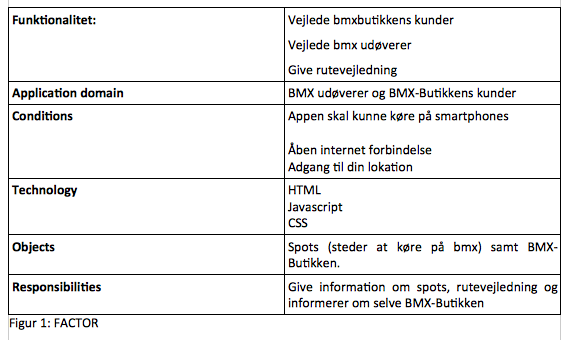
\includegraphics[scale=0.5]{factor.png}
\end{figure}

\pagebreak

\section{Kravspecifikation for IT-løsningen}
(a) De funktionelle og ikke-funktionelle krav til jeres system\\\\
Funktionelle krav:\\
Upload af billeder\\ Uploader billeder fra brugerens enhed, til mysql databasen ved hjælp af php\\
Menu\\ Har ved hjælp af javascript lavet en funktion som viser en ny div øverst på skærmen med indholdet af det pågældende menupunkt, på den måde vil brugeren aldrig blive ført videre til en ny side.\\
Streetspots\\
Skatesparks\\
Markers\\ For hvert spot der bliver loadet fra mysql databasen, bliver der lavet en marker med lidt information om spottet og billeder.\\
Rutevejledning\\ Vejleder brugeren til det pågældende punkt på kortet ved hjælp af google maps.\\
Bruger lokation\\ Finder brugerens lokation vedhjælp af HTML5 og den indbyggede funktion der hedder geolocation, brugeren skal give tilladelse til at programmet må se brugerens lokation.\\
BMX-Butikken\\\\
Ikke funktionelle krav:\\
Appens sprog skal være på engelsk\\ Så den kan bruges af turister, men samtidig af de lokale da de fleste i miljøet snakker engelsk.\\
Bruger venligt UI\\ så alle kan finde ud af at bruge programmet.\\
\pagebreak\\

(b) En use case model, der beskriver system-funktionaliteten. Der ønskes et højniveau-diagram,
som giver overblik over hvilke use cases de forskellige aktører har.\\
\begin{figure}[htb]
\begin{center}
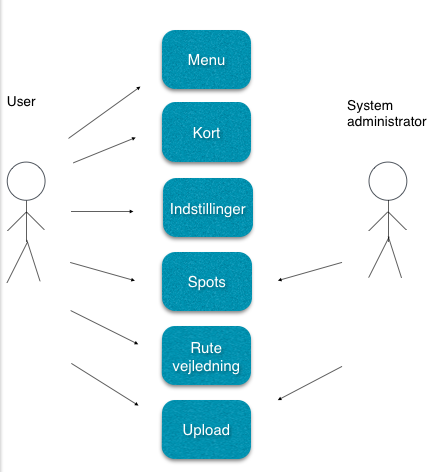
\includegraphics[scale = 0.65]{Umodel}
\end{center}
\end{figure}

Højniveau diagram der skal illustrere de forskellige aktører\\\\
Som det ses er der 2 aktører, brugeren og Ejeren. Brugeren kan benytter de forskellige funktioner i appen, og ejeren redigere og kontrollere uploads og spots. 
\pagebreak\\
(c) Tre specificerede use cases, som er særlig vigtige i jeres system, se fx OOSE figur 4-22.\\
\setlength\parindent{0pt}
\section*{Use-cases}
\subsection*{Få rutevejledning til et spot}
\hrule\vspace{5mm}
\textit{Use case name:} FindSpot\\
\hrule\vspace{5mm}
\textit{Actor:} en bruger der gerne vil finde et spot\\
\hrule\vspace{5mm}
\textit{Entry condition:} brugeren åbner appen\\
\hrule\vspace{5mm}
\textit{Flow of events:}
\begin{enumerate}
\item Brugeren bliver præsenteret for et kort med sin egen positition i centrum og en menu linje i toppen
\item Brugeren trykker på en "marker" på kortet, der sender ham videre til en info side om netop det spot
\item Brugeren trykker på "get directions" og bliver ført til rutevejlednings funktionen med nogle passende ruter
\item Brugeren trykker her på "start" hvorefter kørselsvejledningen starter
\end{enumerate}
\hrule\vspace{5mm}
\textit{Exit condition:} Brugeren ser nu et kort med ruten og får løbende information om hvilken vej denne skal gå\\
\hrule\vspace{5mm}
\newpage
\subsection*{Tilføj spot}
\hrule\vspace{5mm}
\textit{Use case name:} AddSpot\\
\hrule\vspace{5mm}
\textit{Actor:} en bruger der gerne vil tilføje et spot\\
\hrule\vspace{5mm}
\textit{Entry condition:} brugeren åbner appen\\
\hrule\vspace{5mm}
\textit{Flow of events:}
\begin{enumerate}
\item Brugeren trykker på knappen "Add spot", der sender ham videre til en udfyldelses formular
\item Brugeren udfylder formularen og gemmer denne, formularen sendes derefter til godkendelse hos administratoren
\end{enumerate}
\hrule\vspace{5mm}
\textit{Exit condition:} Brugeren sendes retur til forsiden\\
\hrule\vspace{5mm}
\newpage
\subsection*{Ændre indstillinger}
\hrule\vspace{5mm}
\textit{Use case name:} ChangeCondition\\
\hrule\vspace{5mm}
\textit{Actor:} en bruger der gerne vil ændre indstillingerne\\
\hrule\vspace{5mm}
\textit{Entry condition:} brugeren åbner appen\\
\hrule\vspace{5mm}
\textit{Flow of events:}
\begin{enumerate}
\item Brugeren trykker på indstillinger, der sender brugeren videre til en ny side
\item Brugeren bliver præsenteret for de forskellige indstillinger han kan vælge
\item Når brugeren han ændret indstillinger er der en ok knap som tilføjer indstillingerne
\end{enumerate}
\hrule\vspace{5mm}
\textit{Exit condition:} Indstillingerne er nu i funktion og brugeren sendes tilbage til forsiden\\
\hrule\vspace{5mm}
\pagebreak

(d) Et klassediagram over jeres problemområde (solution-domain).\\
\textbf{HJÆLP KASPER!!!!!}\\
(e) Sekvens-diagrammer over de 3 use-cases specificeret i punkt (c).\\
Husk at alle diagrammer skal være fulgt af tekstbeskrivelser, der gør diagrammerne fuldt
forståelige også for læsere uden særligt domænekendskab.\\
\begin{figure}[h]
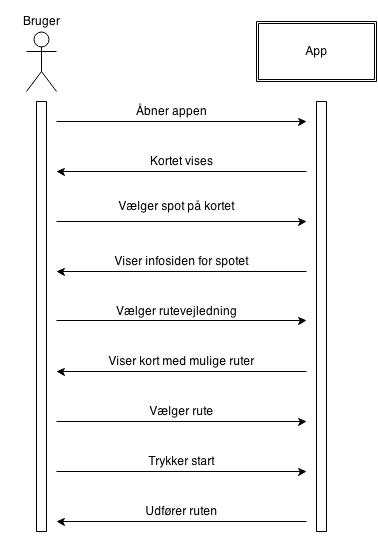
\includegraphics[scale = 0.4]{rutevejledning}
\end{figure}

\begin{figure}[h]
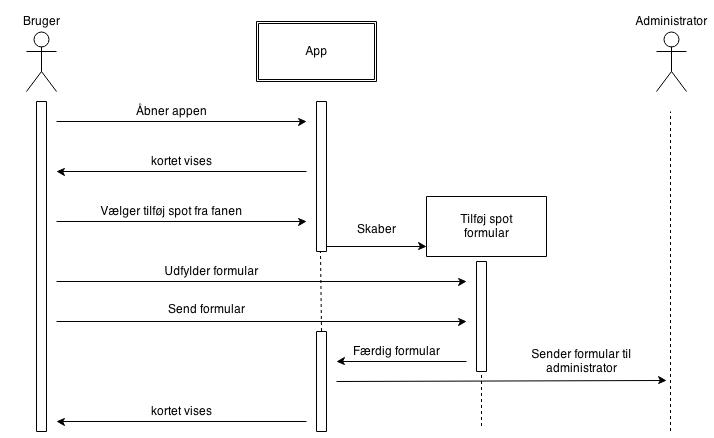
\includegraphics[scale = 0.4]{addspotdia}
\end{figure}

\begin{figure}[h]
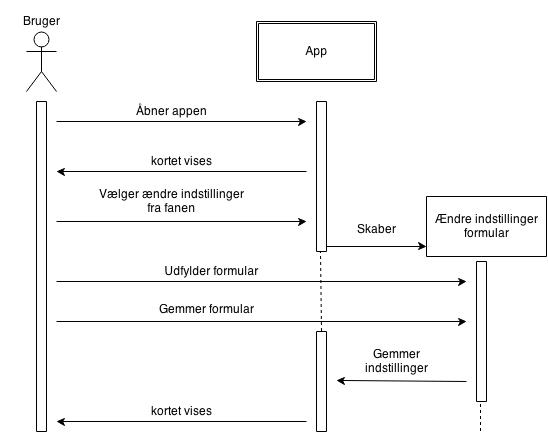
\includegraphics[scale = 0.4]{indstillinger}
\end{figure}


\pagebreak

\section{Systemdesign sammenfatning}
Kapitlet resumerer jeres foreløbige system-design så kort og klart som muligt. Samtidig
udpeger I de vigtigste udestående design- og implementationsopgaver.\\

Vores plan vedrørende udviklingen af appen har indtil nu, været at bygge appen op i java med android developer tools. Det gav os en del udfordring, da vi ikke kunne få den simpleste udgave til at køre på en simulator. De mange timer og forsøg har gjort at vi følte os nødsaget til at gøre projektet mindre omfattende. 
\\\\
Derfor har vi valgt at bygge applikationen op webbaseret i html, css, javascript og mySQL, hvilket er programmer og metoder vi har erfaring med i forvejen. 
Hele implementeringen af Google maps foregår med javascript(altså som en hjemmeside), hvor vi så bagefter vil lave en android webview app, så vi kan tilføje applikationen på google play store. vi mangler at implementere alt andet end kortet på nuværende tidspunkt.

\section{Program- og systemtest}
Dokumenter jeres foreløbige test af IT-løsningen. I kapitlet sammenfattes hovedresultaterne af
jeres test-aktiviteter; mens test plan, test case specification, test incident report og test report
summary placeres som bilag.

\pagebreak
\section{Brugergrænseflade og interaktionsdesign}
(a) Præsenter skærmbilleder af de mest interessante dele af jeres brugergrænseflade.

\begin{figure}[h]
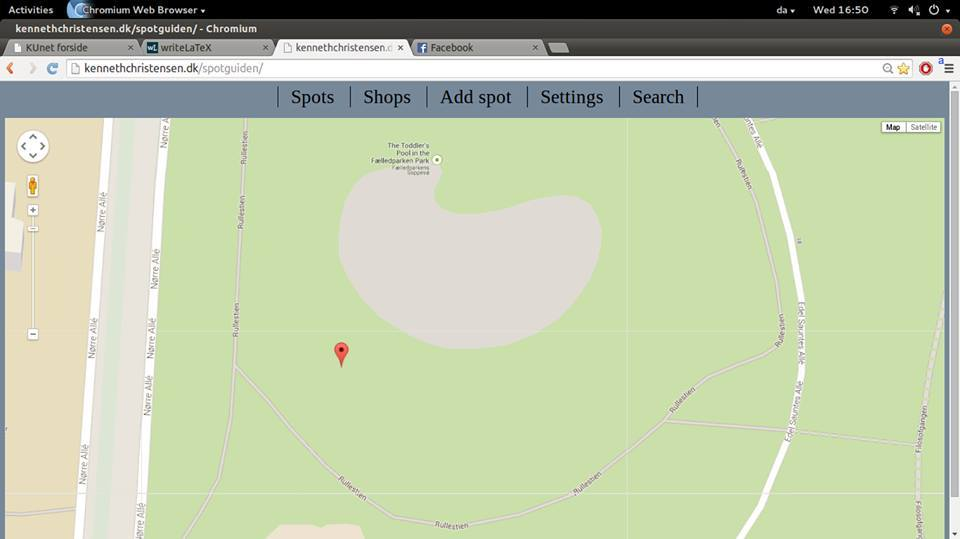
\includegraphics[scale = 0.3]{screen1}
\end{figure}

Billedet viser vores foreløbige hjemmeside der blot indeholder en menu uden funktioner, samt et kort med "spots" på den måde som vi vil præsentere dem. \\ \\
Settings: Når man trykker på settings kommer der en slider, som der kan bestemme hvor stor en radius siden skla loade spots fra, vurderet fra brugerens nuværende position.\\
Spots: Når du trykker her kommer der en liste frem over alle de forskellige spots som man herefter trykke på dem. Dette vil centrerer dem på kortet.\\
Shops: Centrerer kortet på BMXButikken.\\
Add spot: Når der trykkes på dette kommer der en formular frem som man skal udfylde med: Name, Address, City, zip og billede.\\
Search: Kommer frem med et søgefelt hvor man kan søge på spots via navn/zipcode/by.\\

(b) Illustrer flowet/dynamikken i brugerinteraktionen mellem skærmbillederne.\\
Dette vil blive udfyldt i delrapport 3 eller 4 hvor vi er kommet længere med programmet.\\
(c) En audio-visuel præsentation af brugergrænsefladen af den seneste kørende prototype.\\
Formatet vælger I frit, fx en video der illustrerer IT-løsningen med vigtige use cases, en serie
screenshots med speak, slideshow med forklarende tekst. Dog skal det i alle tilfælde afleveres som
et YouTube link og være uploadet som en ”skjult video”.\\
(d) Resultatet af seneste tænke-højt forsøg gennemført med een eller flere af jeres brugere.\\
Dette punkt vil blive udfyldt til delrapport 3 da vi har aftale med flere brugere.\\

\pagebreak
\section{Versionstyring}
Til aflevering: Som bilag skal vedlægges jeres nuværende commit-log samt jeres
programkode. Kommentér kort (ca 1/2 side) de vigtigste ændringer, der er sket i programkoden.\\

Det første udkast til systemet blev skrevet med java/google developer tools som vi havde planlagt det. Men efter mange timers forsøg, måtte vi erkende det måske var en uoverkommelig opgave.\\
Vi er derfor gået over til at lave appen webbaseret og bruge javascript, css, php, html og mySQL til at snakke med en database. Vi har nu fået det opdateret så den finder spots fra databasen. \\
\\
Derudover er vi også gået igang med at lave en app til android som der loader hjemmesiden ned så folk også kan bruge som app hvis de vil det. Denne vil også loade mappet så det ligger på deres telefon så de i princippet også kan bruge kortet uden net, som vil gøre det muligt for dem stadig at se alle spots men ikke kunne tilføje og ændre på indstillinger.




\pagebreak
\section{Projektsamarbejdet}
Til aflevering: Beskriv konkret og oplysende hvordan det går med samarbejdet med brugerne
og med arbejdet internt i gruppen. Herunder skal bl.a. oplyses antallet af møder med brugerne under
projektforløbet (fx på en tidslinje), mødeformen i gruppen, samt hvorledes jeres referat- og
dokumentationsform fungerer. Hvorledes prioriterer og styrer I projektindsatsen, så I sikrer
fremdrift på de felter, som er mest risikable/afgørende for et succesfuldt resultat? Herunder, beskriv
og diskuter:\\

(a) Hvad går godt?\\
Det interne arbejde i gruppen fungerer godt. Alle medlemmer i gruppen deltager aktivt, engageret og møder til tiden på de aftalte møde dage. Selve arbejdet prøver vi at fordele imellem os alt efter interesse og det sikrer en god stabil arbejds indsats.\\

(b) Hvad går mindre godt?\\

Vi har haft uventede problemer hvad angår systemdesignet da vi har måttet ændre kurs og gå over i en webbaseret udgave. Det har betydet at vi har haft nogle arbejdsspildtimer og vi er derfor ikke noget helt så langt som planlagt.\\

(c) Hvad vil I gøre for at effektivisere jeres udviklingsarbejde?\\

I det vi tog skridtet fra android app til webbaseret app, har vi taget de første skridt i effektiviseringen. Derudover regner vi med at kunne begynde at arbejde selvstændigt på enkelte dele af systemet når vi har fået den første prototype helt op at køre. Det skullle bevirke at det bliver nemmere for de enkelte individer i gruppen at få plads i deres skema, til at få arbejdet på projektet og dermed få arbejdet flere timer. 

\pagebreak
\section{Review}
\subsection{Designing for usability}
Artiklen omhandler metoder for en programmør til at fuldfører IT-projekter, der ender ud med at have en høj værdi af "usability" (Nemt og intuitivt for slutbrugeren at benytte). Det handler primært om 3 teoretiske systemudviklings metoder, som ophavsmændene til artiklen mener man bør følge for at udvikle et nemt og brugbart computer system. De 3 metoder er: "Early and continual focus on users", "empirical measurement of usage" and "iterative design". \\\\
Early and continual focus on users\\
Handler om at designerne skal forstå hvem slutbrugerne er. Det betyder at designerne skal studere brugernes arbejde og evaluerer på hvordan bruger interagere med systemet.\\\\
Empirical measurement of usage\\
Går ud på at der i udviklings processen skal indlægges tid til at lave slutbruger undersøgelser. Konkret betyder det at der i processen skal udvikles prototyper, som slutbrugeren kan benytte til at udføre deres faktiske arbejde. Brugeren skal så observeres og processen skal analyseres for at forbedre prototypen.\\\\
Iterative design\\
Går ud på at når brugerne finder en fejl under en test, skal fejlene udbedres. Det betyder så at produktet skal igennem en ny design fase, testing, "measurement". Disse 3 faser gentages så ofte som dette måtte være nødvendigt for at opnå det ønskede niveau af funktionalitet, brugervenlighed og hvad man ellers måtte prioritere.
\\\\
Resten af artiklen omhandler disse 3 teoretiske metoder i forhold til virkeligheden. Der lægges vægt på at de nævnte metoder virker intuitive for en programmør/designer når de bliver læst højt, men flere tests viser at metoderne måske ikke er så intuitive alligevel. Undersøgelsen viser nemlig at meget få mener at netop disse metoder er nogle af de hovedpunkter man skal overveje når man skal udvikle og evaluere et nyt system. \\\\Derudover sammenlignes denne protokol også med andre som "get it right, the first time" og deciderede design guidelines. \\\\
Konkret bliver det pointeret at det er stortset umuligt at "get it right the first time", det ville nemlig indebære at der var blevet lavet et perfekt systemdesign fra starten, samt at man ignorede eventuelle erfaringer man gjorde sig om brugeren og systemet undervejs i projektet. Generelle guidelines ses som værende ufuldstændige og problematiske. Hvilket kommer af at design guidelines netop er generelle og altså ikke tager højde for nogen konkrete situationer der måtte opstå og derfor kommer designeren til at skulle træffe de fleste beslutninger selv.\\\\
Det vi i gruppen mener der er værd at tage med fra denne artikel er selve ideen om at gøre et system brugervenligt, nemt og intuitivt. Vi er enige om at et gennemført system der er nemt at bruge, er et system der i højere grad vil blive brugt. For at trække paraleller til vores eget projekt, så har vi indtil videre kun været i tæt dialog omkring funktionalitet med vores kunde og ikke snakket meget om selve systemets interface. Dermed må vi også erkende at selvom metoderne nu virker intuitive, oplagte og at netop disse metoder er blevet prædiket flere gange til forskellige forelæsninger, endda i forskelle fag. Så er metoderne alligevel ikke kommet intuitivt og vi må derfor bestræbe os på at få en dialog igang med nogle slutbrugere, der kan evaluere på vores foreløbige systemdesign og måske forbedre det. På den måde kan vi implementere de 3 metoder og få gang i en "design, test og evaluerings" cyklus og løbende forbedre vores system imens vi nærmer os et slutprodukt.\\\\
\pagebreak

 \subsection{A rational design process: How and why to fake it.}

Artiklen handler om den ideelle måde at designe programmer på. Den er delt i 3 nogenlunde klare dele. Første del omhandler den ideelle rationale designproces og hvorfor den ikke kan opnås. Anden del er forfatternes eksempel på en designproces. Og trejde del omhandler styrken af forfatternes designproces mod nutidige metoder.\\\\
Den ideelle designproces\\
Artiklen starter ud med at fortælle om den ideelle rationale designproces, hvor en designproces næsten kan sammenlignes med et matematiske bevis, hvor i man kan følge en logisk tråd fra start til slut. Herefter klargører den hvorfor dette stort ser ikke er en mulig måde at udføre designprocessen på. Artiklen argumentere at de logiske skridt ikke kan følges f.eks pga. kravende til programmet kan ændre sig løbende eller at menneskelige fejl opstår. Efterfølgende forklares hvorfor det er god ide at tilnærme sig en sig en sådan designproces, selvom den ikke er mulig at opnå.\\\\
Designproces eksemplet\\
Artiklen udlægger herefter et eksempel på en rationel designproces man kan bruge. Gennem 7 punkter forklares der hvordan man skal dokumentere og sørge for at kravende er gode for designprocessen, hvordan man skal bryde programmet ned i moduler som er overkommelige og sørge for modulernes indbyrdes funktioner. Det forklares at stort set hele processen er dokumentation som klargører hvad der skal gøres, og at det derfor er nemmere at lave de logiske rationalle skridt som skal tages.\\\\
Forfatternes proces mod nutidige metoder\\
Til sidst forklarer artiklen om nutidig dokumentation og problemerne ved det. Nutidig dokumentation lider under at programmøre betragter dokumentation som noget overflødigt, og derfor er dokumentationen ukomplet og upræcis. Derefter slås det fast hvor vigtig god dokumentation er for den ideelle designprocess.\\\\ \pagebreak\\
Det vi i gruppen mener der er værd at tage med fra denne artikel er selve ideen om at bruge en designproces, som nærmer sig den logiske og rationelle proces der er beskrevet i starten af artiklen. Hvis man kan finde en nogenlunde standart måde at design sine programmer er det helt klart fordelagtigt. Eksemplet der er beskrevet virker meget gennemtænkt og brugbart. Designprocessen foreslået i artiklen ligner meget den proces som vi skal bruge i vores delrapporter. Det ligner også meget det som er blevet gennemgået i vores undervisning og vi forsøger at følge den efter bedste formåen.

\newpage

\section{Bilag}

\subsection{Commitlog}
* <3db9ac0> 2014-05-07 [rasmus03]  Opdaterede tekst i delrapport 2\\
* <b4614f0> 2014-04-28 [mhejselbak]  CSS til hjemmeside\\
* <d0c4133> 2014-04-28 [rasmus03]  Tilføjede første udlæg til den webbaserede android application - Ingen test af funktioner muligt \\
* <ba05d40> 2014-04-28 [rasmus03]  Tilføjede vores review af “Mood”\\
* <1da40ab> 2014-04-24 [rasmus03]  Updaterede filer til delrapport 2\\
* <89ae7a4> 2014-04-24 [rasmus03]  Commitlog billede\\
* <6f57d2e> 2014-04-24 [rasmus03]  Tilføjede vores udkast til hjemmesiden - Ingen implementeringer\\
* <2077057> 2014-04-24 [runefranch]  Nyt sekvens dia\\
* <a006ca4> 2014-04-24 [runefranch]  sidste sekvens dia\\
* <f2ad5a2> 2014-04-23 [rasmus03]  Updated files and added screenshots\\
* <c201cd9> 2014-04-23 [runefranch]  sekvens diagram\\
* <ee33ad2> 2014-04-23 [rasmus03]  Opdaterede delrapport2 med 2/2 review og use-cases. Standard clean up af unødige filer\\
* <592de43> 2014-04-23 [runefranch]  reviewartikel\\
* <e77b576> 2014-04-23 [rasmus03]  FACTOR model - Bruges i delrapport 2\\
* <599276d> 2014-04-23 [rasmus03]  Delrapport 2 - Består af punkt 1, 2 og 1/2 review\\
* <b2271ec> 2014-04-22 [mhejselbak]  Prototype\\
* <6e1b71b> 2014-04-10 [runefranch]  review update\\
* <d81beae> 2014-04-09 [runefranch]  Review\\
* <19705bc> 2014-04-03 [mhejselbak]  Initial commit\\
\end{document}


